% \documentclass{article}
% \usepackage{graphicx}
% \usepackage{url}
% \usepackage[utf8]{inputenc}
%\usepackage[margin=1in]{geometry}

% \begin{document}
% \title{Aaron McKay - Research and Background}
% \author{Aaron McKay}
% \maketitle

% Above lines are commented by Marwan Alharbi, since this is sub-latex file related to main one (Assignment3-git.tex) so no need to include latex header here

% Your content from first assignment
\section{Aaron McKay}
I am a 2nd year PhD student at UCCS.  I haven't yet published a paper but I'm working on it.  My area of research I think is one of the most challenging in all of cybersecurity, Cyber Risk Quantification (CRQ).  Its taken me some time to figure out how this problem is best approached and I think the answer lies in a deep classification and analysis of the interactions of Attackers and Defenders. There may be several derivations from this interaction, but since my attention is on cyber risk quantification, my focus is on "Susceptibility" of Systems and Users not only as a metric but as a factor to be used upstream the CRQ calculations.

\begin{figure}[h]
    \centering
    
\includegraphics[width=0.5\textwidth]{images/Oh_Yeah.jpg}
    \caption{Oh Yeah}
    \label{fig:oh-yeah}
\end{figure}

\section{Research Code Experience}
\subsection{Repository Used and Implementation Decisions}
I explored the Netflix-Skunkworks RiskQuant repository 
(\url{https://github.com/Netflix-Skunkworks/riskquant}). While attempting to use 
the full repository, I encountered compatibility issues with numpy<1.19.0,>=1.16.0 
when trying to install with Python 3.12. Rather than downgrade Python, I decided to 
implement a simplified version focusing on the core risk quantification concepts.

The simplified implementation used Python's built-in libraries:
\begin{itemize}
    \item random: for Monte Carlo simulation
    \item statistics: for statistical analysis
    \item Python classes: to organize the risk model structure
\end{itemize}

\begin{figure}[h]
    \centering
    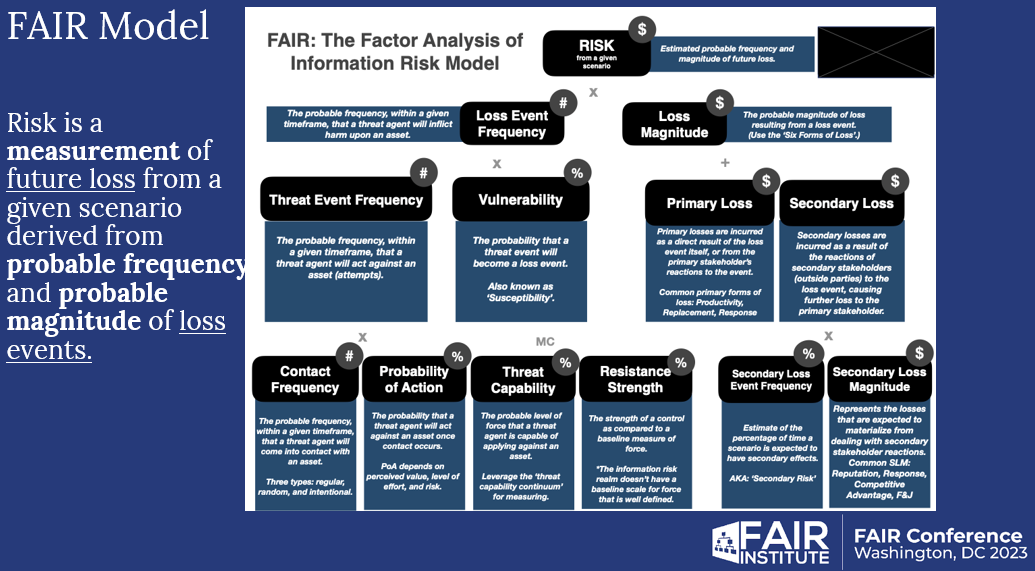
\includegraphics[width=\textwidth]{images/fair_model.png}
    \caption{FAIR (Factor Analysis of Information Risk) Model presented at FAIR Conference 2023, Washington, DC. The FAIR model is a popular implementation of CRQ.
    Credit: Jon Baker (Co-founder \& Director, Center for Threat-Informed Defense), 
    Arvin Bansal (vCISO, Fortune500), and Vidit Baxi (Co-founder \& CISO, Safe Security)}
    \label{fig:fair-model}
\end{figure}

\subsection{Testing Experience and Implementation Details}
I created a SimpleRiskModel class that implements Monte Carlo simulation to estimate 
potential losses from cyber incidents. The model was designed with these key components:
\begin{itemize}
    \item Class initialization with risk parameters (min loss, max loss, probability)
    \item Simulation method running 10,000 iterations
    \item Analysis method calculating key statistics
    \item Output formatting for clear result presentation
\end{itemize}

The testing process involved:
\begin{enumerate}
    \item Setting up a data breach scenario with realistic parameters
    \item Running multiple simulations to verify consistency
    \item Analyzing the distribution of results
    \item Validating that the average loss aligned with theoretical expectations
\end{enumerate}

Key model parameters were chosen based on typical cyber incident statistics:
\begin{itemize}
    \item Minimum loss: \$100,000 (typical small breach cost)
    \item Maximum loss: \$1,000,000 (potential major incident)
    \item Annual probability: 10\% (industry average for similar incidents)
    \item Iterations: 10,000 (for statistical significance)
\end{itemize}

\subsection{Output Examples}
\begin{verbatim}
Risk Analysis for Data Breach Scenario:
Average Annual Loss: $52,624.65
Maximum Potential Loss: $999,737.69
90th Percentile Loss: $0.00
\end{verbatim}

\subsection{Analysis}
The results show an average annual loss of about \$52,600, which aligns with the 
10\% probability of an incident occurring. The maximum potential loss approaches 
the upper limit of \$1,000,000, demonstrating the model's ability to capture 
worst-case scenarios. The 90th percentile being \$0 indicates that in most 
simulation runs (over 90\%), no loss occurred, which is consistent with the 
low probability of occurrence.

\section{Merge Conflict and Permission Resolution}
During this assignment, I encountered two significant challenges that required resolution:

\subsection{Repository Permission Issues}
Initially, I was unable to push my changes to the repository due to permission restrictions. I attempted several approaches:
\begin{enumerate}
    \item First tried pushing directly using HTTPS protocol (received 403 error)
    \item Attempted using SSH authentication
    \item Created a fork of the repository as a backup
    \item Generated a patch file (mckay-changes.patch) to preserve my changes
    \item Finally resolved when Dr. Boult granted proper repository access
\end{enumerate}

\subsection{Merge Conflicts}
After gaining proper access, I encountered merge conflicts when trying to merge upstream/main into my branch. 
The conflicts involved two files (cardenas.tex and jcastanonremy.tex) that were deleted in my branch 
but modified in upstream/main. I resolved these conflicts by:
\begin{enumerate}
    \item First checking the status using git status to understand the nature of the conflicts
    \item Using git rm --cached to remove the conflicting files from Git tracking
    \item Committing the resolution with an appropriate commit message
    \item Cleaning up the working directory by removing the untracked files
    \item Successfully completing the merge afterward
\end{enumerate}

This experience helped me understand both the importance of proper repository permissions and 
how to handle conflicts between different branches in a Git repository. It demonstrated 
real-world scenarios of collaboration challenges and their solutions.

\section{Questions and Answers}
% This section will be used later for Q&A
\begin{enumerate}
    \item How do you plan to improve your Monte Carlo simulation model to handle more complex cyber attacks or different types of attackers in the future?
    
    \subsection*{Answer}
The current Monte Carlo simulation model provides a basic framework for risk quantification, 
    but there are several planned improvements to handle complex attack scenarios:
    
    \begin{itemize}
        \item Incorporate attacker profiles with different skill levels, resources, and motivations
        \item Add multi-stage attack modeling to capture attack chains and dependencies
        \item Include temporal factors to model how risks evolve over time
        \item Integrate the FAIR model's components more explicitly, especially the 'Threat Event Frequency' 
              and 'Vulnerability' factors shown in the diagram
        \item Add correlation between different types of attacks to model complex scenarios
        \item Implement Bayesian updating to refine probabilities based on observed incidents
    \end{itemize}
    
    The goal is to move beyond simple probability-based scenarios to a more nuanced model that 
    reflects the dynamic nature of cyber threats while maintaining computational efficiency.
\end{enumerate}


% \end{document}